\documentclass[UTF8]{report}
\usepackage{ctex}
\usepackage{graphicx}
\usepackage{subfigure}

\begin{document}
    \section*{1.}
        由题意得,$f_X(x) = \frac{1}{2}$,所以
        $F_Y(y) = P(Y \leq y) = P(\sqrt{|X|} \leq y) = P(|X| \leq y^2)$。

        $$F_Y(y) = \left\{
            \begin{array}{lcr}
                y^2 & & y \in [0, 1]\\
                0 & & otherwise
            \end{array}
        \right.$$

        求导后即可得到:
        $$f_Y(y) = \left\{
            \begin{array}{lcr}
                2y & & y \in [0, 1]\\
                0 & & otherwise
            \end{array}
        \right.$$

        因为$F_Z(z) = P(Z \leq z) = P(-ln|X| \leq z) = P(|X| \geq e^{-z})$

        $$F_Z(z) = \left\{
            \begin{array}{lcr}
                1 - e^{-z} & & z \in [0, \infty]\\
                0 & & otherwise
            \end{array}
        \right.$$

        所以
        $$f_Z(z) = \left\{
            \begin{array}{lcr}
                e^{-z} & & z \in [0, \infty]\\
                0 & & otherwise
            \end{array}
        \right.$$
    \section*{2.}
        令$Y = e^X$,则$F_Y(y) = P(Y \leq y) = P(e^X \leq y) = P(X \leq lny)$,
        所以$F_Y(y) = \int_{-\infty}^{lny}f_X(x)dx$,求导后$f_Y(y) = \frac{f_X(lny)}{y}$。

        当X服从$[0, 1]$上的均匀分布时:
        $$f_Y(y) = \left\{
            \begin{array}{lcr}
                \frac{1}{y} & & y \in [1, e]\\
                0 & & otherwise
            \end{array}
        \right.$$
    \section*{3.}
        令$Y = |X|^{\frac{1}{3}}, Z = |X|^{\frac{1}{4}}$,则:
        $F_Y(y) = P(Y \leq y) = P(|X|^{\frac{1}{3}} \leq y) = P(|X| \leq y^3) = \int_{0}^{y^3}f_{|X|}(|x|)dx$,
        所以$f_Y(y) = 3y^2f_{|X|}(y^3)$,同理$f_Z(z) = 4z^3f_{|X|}(y^4)$。
    \section*{4.}
        因为$F_Y(y) = P(Y \leq y)$,当$0 \leq y \leq 5$时,由全概率公式,
        $P(Y \leq y) = \frac{1}{4}P(X \leq y) + \frac{3}{4}P(X - 5 \leq y) = \frac{1}{4}P(X \leq y) + \frac{3}{4}P(X \leq y + 5)$,
        所以$P(Y \leq y) = \frac{1}{4}(\int_{0}^{y}f_{X_A}(x)dx + 3\int_{0}^{y + 5}f_{X_B}(x)dx) = \frac{y}{10} + \frac{1}{4}$,故$f_Y(y) = \frac{1}{10}$;
        同理当$5 < y \leq 15$时,$P(Y \leq y) = \frac{3}{4}\int_{0}^{y + 5}f_{X_B}(x)dx = \frac{y + 5}{20}$,所以$f_Y(y) = \frac{1}{20}$。
    \section*{5.}
        \begin{figure}[h]
            \centering
            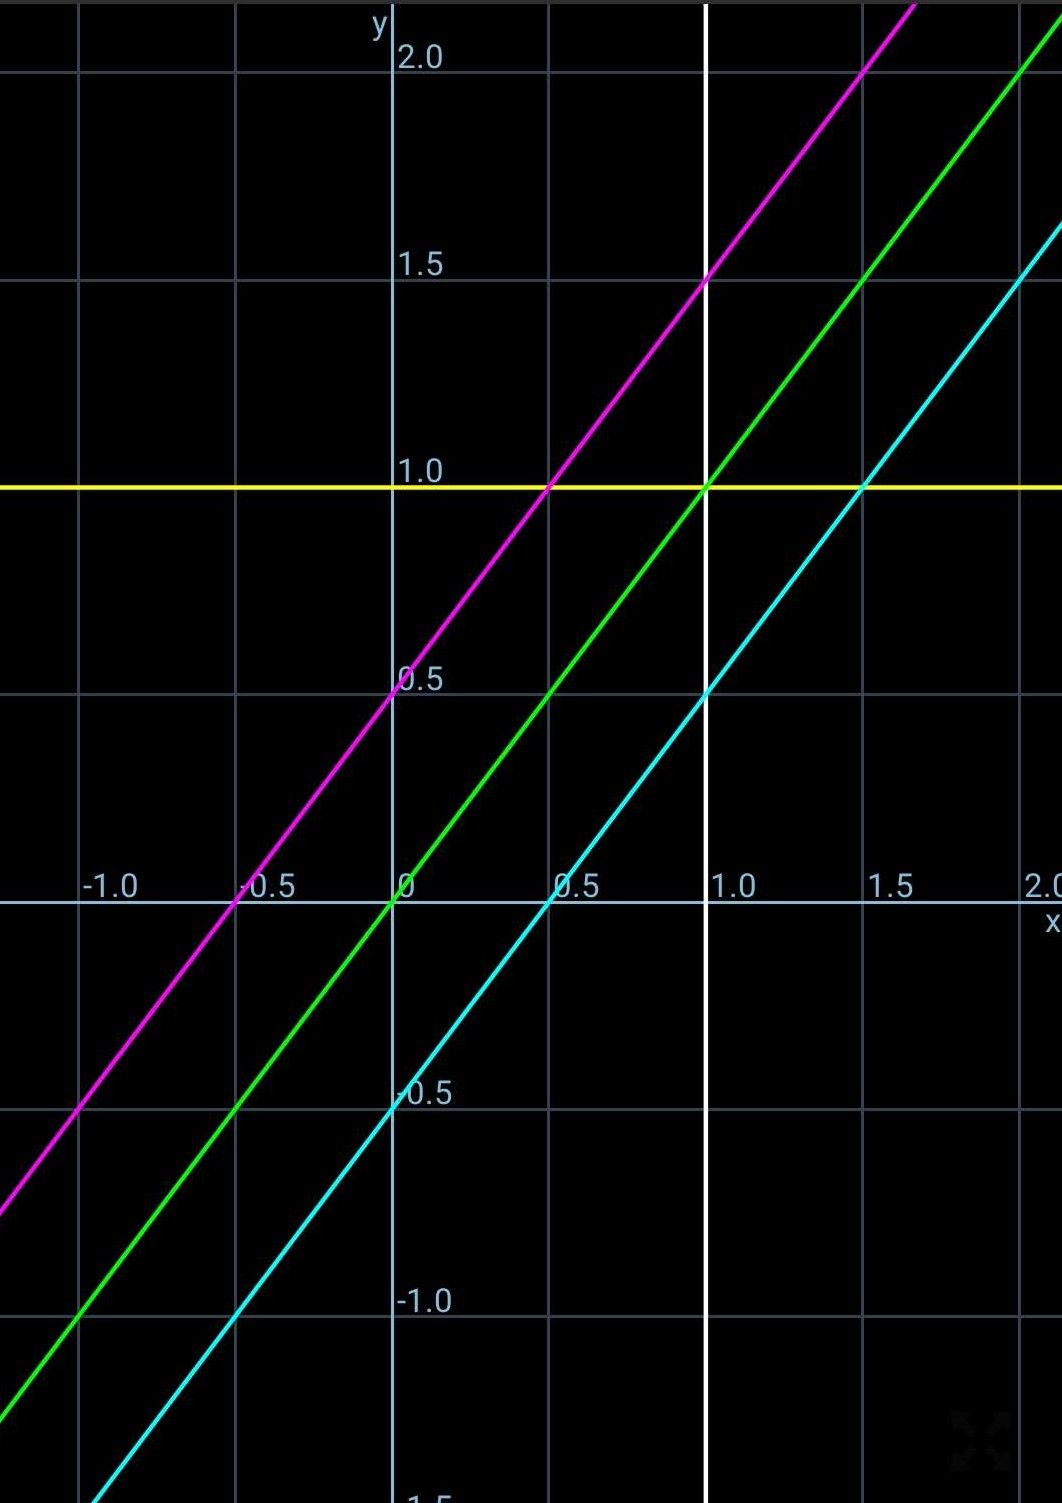
\includegraphics[width=4cm, height=5cm]{img4-1-5.jpg}
            \caption{$|z| = 0.5$的情况}
        \end{figure}

        由于$X, Y$均服从均匀分布,两个随机变量的联合概率可以用以上的正方形区域面积表示。
        考虑$|X - Y| \leq z$,这个式子可以被拆开为两个式子$X - Y \leq z$和$Y - X \leq z$,在图中做出这两个函数的图像。
        不难发现$P(Z \leq z)$就是两条平行线与正方形所包围的图形的面积,即$P(Z \leq z) = 2z - z^2$,所以$f_Z(z) = 2 - 2z$。
    \section*{6.}
        使用和第五题类似的做法:$P(Z \leq z) = P(|X - Y| \leq z) = \frac{\sqrt{2}z}{2}(\sqrt{2}z + \frac{\sqrt{2}}{2}(1 - z) * 2) = \frac{z}{2}$,
        所以$f_Z(z) = \frac{1}{2}$。
    \section*{7.}
        不难看出这题的随机变量就是第五题中的Z。所以$E[Z] = \int_{0}^{1}2z^2 - z^3dz = \frac{1}{3}$。

        证毕。
    \section*{8.}
        $$f_Z(z) = \int_{-\infty}^{\infty}f_X(x)f_Y(z - x)dx = \int_{0}^{z}\lambda^2e^{-\lambda x}e^{-\lambda (z - x)}dx = \lambda^2ze^{-\lambda z}$$
    \section*{9.}
        当$z \leq 0$,
        $$\begin{array}{l}
            F_Z(z) = P(X - Y \leq z) = 1 - P(X - Y > z)\\
            = 1 - \int_{0}^{\infty}\mu e^{-\mu y}dy\int_{z + y}^{\infty}\lambda e^{-\lambda x}dx\\
            = 1 - \frac{\mu}{\lambda + \mu}e^{-\lambda z}
        \end{array}$$

        当$z < 0$时,$-z \leq 0$,所以$F_Z(z) = 1 - F_Z(-z) = \frac{\mu}{\lambda + \mu}e^{\lambda z}$。
    \section*{10.}
        由离散卷积公式$f_Z(z) = \sum f_X(x)f_Y(z - x)$可以求得:
        $$p_Z(z) = \left\{
            \begin{array}{lcr}
                \frac{1}{6} & & z = 1\\
                \frac{5}{18} & & z = 2\\
                \frac{1}{3} & & z = 3\\
                \frac{1}{6} & & z = 4\\
                \frac{1}{18} & & z = 5
            \end{array}
        \right.$$
    \section*{11.}
        设$P_X(k) = e^{-\lambda}\frac{\lambda^k}{k!}, P_Y(k) = e^{-\mu}\frac{\mu^k}{k!}$,
        由卷积公式,有$P_Z(z) =\\ \sum P_X(k)P_Y(z - k)$,因为$C_z^k = \frac{z!}{k!(z - k)!}$,
        所以$P_Z(z) = \frac{e^{(-\lambda + \mu)}}{z!}\sum C_z^k \lambda^k \mu^{z - k}\\ = e^{-(\lambda + \mu)}\frac{(\lambda + \mu)^z}{z!}$。

        证毕。
    \section*{12.}
        先求$W = X + Y$的概率密度函数:
        $$f_W(w) = \left\{
            \begin{array}{llccr}
                \int_{0}^{w}dx & = & w & & 0 \leq w \leq 1\\
                \int_{w - 1}^{1}dx & = & 2 - w & & 1 < w \leq 2\\
                0 & & & & otherwise
            \end{array}
        \right.$$

        再求$R = W + Z$:
        $$f_R(r) = \left\{
            \begin{array}{llccr}
                \int_{0}^{r}wdw & = & \frac{r^2}{2} & 0 \leq r \leq 1\\
                \int_{r - 1}^{1}wdw + \int_{1}^{r}2-wdw & = & 3r - r^2 - \frac{3}{2} & 1 < r \leq 2\\
                \int_{r - 1}^{2}2 - wdw & = & \frac{r^2}{2} - 3r + \frac{9}{2} & 2 < r \leq 3\\
                0 & & & otherwise
            \end{array}
        \right.$$
    \section*{13.}
        因为概率密度函数的对称轴为$\frac{a + b}{2}$,所以有$f(x) = f(a + b - x)$,
        而$X + Y$和$X - Y$的积分区间正好差着$a + b$的距离,所以只需要将$f_{X + Y}$平移即可。
    \section*{14.}  
        $$\begin{array}{l}
            P_Z(z) = P(min\{X, Y\} \leq z)\\
            = 1 - P((min\{X, Y\} > z)\\
            = 1 - P(X > z)P(Y > z)\\
            = 1 - (1 - P(X \leq z))(1 - P(Y \leq z))\\
            = 1 - (1 - \int_{0}^{z}\lambda e^{-\lambda x}dx)(1 - \int_{0}^{z}\mu e^{-\mu y}dy)\\
            = 1 - e^{-(\lambda + \mu)z}
        \end{array}$$

        所以$Z = min\{X, Y\}$服从参数为$\lambda + \mu$的指数分布。

        证毕。
    \section*{15.}
        略。
    \section*{16.}
        略。
\end{document}